%%%%%%%%%%%%%%%%%%%%%%%%%%%%%%%%%%%%%%%%%%%%%%%%%%%%%%%%%%%%%%%%%%%%%%%%%%%%%%%%
\documentclass[twocolumn]{revtex4}

%%%%%%%%%%%%%%%%%%%%%%%%%%%%%%%%%%%%%%%%%%%%%%%%%%%%%%%%%%%%%%%%%%%%%%%%%%%%%%%%
% Note that comments begin with a "%" and are not turned into text in the .pdf
% document.
%%%%%%%%%%%%%%%%%%%%%%%%%%%%%%%%%%%%%%%%%%%%%%%%%%%%%%%%%%%%%%%%%%%%%%%%%%%%%%%%

%%%%%%%%%%%%%%%%%%%%%%%%%%%%%%%%%%%%%%%%%%%%%%%%%%%%%%%%%%%%%%%%%%%%%%%%%%%%%%%%
% Include some extra packages.
%%%%%%%%%%%%%%%%%%%%%%%%%%%%%%%%%%%%%%%%%%%%%%%%%%%%%%%%%%%%%%%%%%%%%%%%%%%%%%%%
\usepackage[]{graphicx}
\usepackage{amsmath} % % Note: any LaTeX tricks used not taught in class are from this wonderful site - https://www.sharelatex.com/
\usepackage{float}
%%%%%%%%%%%%%%%%%%%%%%%%%%%%%%%%%%%%%%%%%%%%%%%%%%%%%%%%%%%%%%%%%%%%%%%%%%%%%%%%

%%%%%%%%%%%%%%%%%%%%%%%%%%%%%%%%%%%%%%%%%%%%%%%%%%%%%%%%%%%%%%%%%%%%%%%%%%%%%%%%
\begin{document}

%%%%%%%%%%%%%%%%%%%%%%%%%%%%%%%%%%%%%%%%%%%%%%%%%%%%%%%%%%%%%%%%%%%%%%%%%%%%%%%%
\title{
Calculating Rainfall
}

\author{C.~Premo}
%\author{R.~Feynman}
\affiliation{Siena College, Loudonville, NY}

\date{\today}

\begin{abstract}
    %Your abstract is a 1 paragraph summary of the project.
    %You should summarize the motivation, the procedure, and the 
    %results here.
The goal of this final project was to predict rainfall through \textit{numerical} means or through a monte carlo approach. For the first problem, a analytical approach was used also to show that it was in fact a solvable number or probability. The results from the monte carlo approaches were within a certain range from the actual values as expected from the in-class lab we did on numpy and the birthday problem.
\end{abstract}

\maketitle
%%%%%%%%%%%%%%%%%%%%%%%%%%%%%%%%%%%%%%%%%%%%%%%%%%%%%%%%%%%%%%%%%%%%%%%%%%%%%%%%
\section{Introduction}
Monte Carlo approaches allow scientists to calculate more accurate probabilities over a long amount of numbers that cannot possibly be done without code. This final project allows physics majors to see real world application in code through predicting rain-fall. It also provides a good amount of experience with the numpy code and its functionality. 

%%%%%%%%%%%%%%%%%%%%%%%%%%%%%%%%%%%%%%%%%%%%%%%%%%%%%%%%%%%%%%%%%%%%%%%%%%%%%%%%
\section{Problem 1 - Analytic Approach}

Problem 1 asked us to write out a analytic approach in addition to the Monte Carlo method. A certain formula was used to calculate the probability it will rain on one day in the given month of 30 days: \begin{equation} \label{bi_di} p = n * p(x)^{n-1} \end{equation} In this case, n = given number of days in a month, p = probability it will rain, and x = probability it won't rain. With some research, the formula used is also known as the \textit{binomial distribution formula}\footnote{http://www.statisticshowto.com/binomial-distribution-formula/}.

This equation was formulated through the idea that we wanted it to rain on one day. Here is the logic: We want it to rain on \textbf{one day} in a month. To get the probability of it raining one day in a month of 30 days and not the others, let's pick a day. Let's say the day we picked is Sunday, we want it to rain on Sunday *and* not on Monday and *not* on Tuesday etc. We will do this for every day in a week until we reach 30 days to make sure we have each probability for each day. It can be said that each day has the same probability of it raining on only that day, so we would simply multiply the number of days we are given by the probability it will rain on by the probability it won't rain, which is raised to the 29th power as there are 29 days it won't rain in this scenario. Thus the equation \ref {bi_di} is formed. Mathematically, we are given the probability it will rain on any given day in a month, which is 20 percent or 0.20. To find the percentage/probability of it not raining, we would subtract that percentage/probability from 100 percent or just 1. The probability of it not raining is then 80 percent or 0.80. Let's plug what we know into equation \ref{bi_di} to get the probability of it raining one day in a month of 30 days. \begin{equation} 30 * 0.20 * (0.80)^{29} = 0.00928455029464 \end{equation}

Having the answer, we will want to use numpy to create a simulation that gives us a similar probability as it is tested multiple times in python; much like the birthday problem shown in class.

%%%%%%%%%%%%%%%%%%%%%%%%%%%%%%%%%%%%%%%%%%%%%%%%%%%%%%%%%%%%%%%%%%%%%%%%%%%%%%%%
\section{Monte Carlo Approaches}

\subsection{Problem 1}
We are given the probability it could rain in a month of 30 days. With that information, I defined a function "rain()" to test whether it rains or not given the probability of 1/5. From there I defined another function called "month()" that looped over my "rain()" function 30 times to simulate a month. After a month was simulated I then defined the number of months as being equal to 10000 and looped through my "month()" function 10000 times and kept a count when month() was \textbf{equal} to 1 aka the number of times it rained in that month. So if it only rained once in that month, I would add that to the count. After the conditional the probability was found through taking the amount of times a month had 1 day and dividing it by the number of months I tested and then multiplying that answer by 100 to find percentage.
\subsection{Problem 2}
We are again given the probability it could rain in a month of 30 days. With that information, I defined a function "rain()" to test whether it rains or not given the probability of 1/10. From there I defined another function called "month()" that looped over my "rain()" function 30 times to simulate a month. After a month was simulated I then defined the number of months as being equal to 10000 and looped through my "month()" function 10000 times and kept a count when month() was \textbf{greater than or equal} to 8 aka the number of times it rained in that month. So if it rained atleast 8 times in that month, I would add that to the count. After the conditional the probability was found through taking the amount of times a month had \textit{at least} 8 days and dividing it by the number of months I tested and then multiplying that answer by 100 to find percentage.
\subsection{Problem 3}

\subsubsection{a}
For Problem 3, part a;  we have to find the percent of months that contain rainfall greater than or equal to 10cm. I first defined a function "rain\_fall()" that found the amount of rainfall depending upon the probability of the rainfall, given that the percentages add up to 100 percent and the distance between each conditional is unequal, there must be if statements that account for these unequal distances and that add up to 100 percent much like the excercise containing hints for the final project. An example of an if statement: "If a random number between 0 and 1 is greater than or equal to 0 and the random number is less than .2 the rainfall is 1cm". I would do this for each probability given until the rain fall is 5cm or the percentages get to 100 percent.

After that I defined a function that determined if it rained or not given the number of days before it that rained. If it is the first day of the month there is a .1 chance that it will rain and so on. I went from it being the first day of the month to the day being greater than 3 and the probability of it raining if the 3 or more days before it rained. 

Proceeding to the final function, I looped through my "doesitrain()" function 30 times to simulate a month. If it rained \textit{at least} 1 day than I would keep count of the amount of rainfall from my "rain\_fall()" function. After that function was complete I created a variable for the number of months and looped through my "month()" function 10000 amount of times and kept count of when the rainfall given by the "month()" function was at least 10cm. To find the probability I simply divided the number of times this occurred and multiplied by 100 to find percentage.
\subsubsection{b}
Now I plotted the amount of rainfall using my "month()" function vs. the number of times this occurred or "10000 months". The "month()" function was appended to a list that was used in the "plt.hist()" function. I adjusted the bins and range to bring the amount of rainfall and number of occurences into a more reader-friendly view.

\begin{figure}[H]
    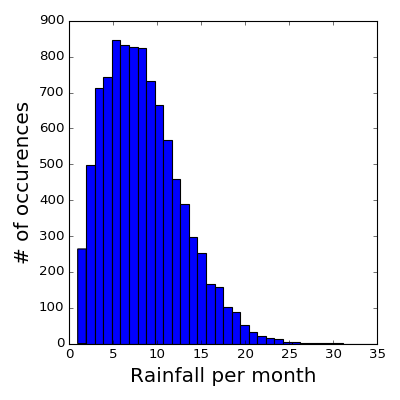
\includegraphics[width=0.45\textwidth]{hist_plot.png}
    \caption{Amount of rainfall vs. Number of occurrences}
\end{figure}
\subsubsection{c}
In part c the average amount of rain in any given month was found through using the "numpy.mean" function taking in the amount of rainfall over the amount of months generated, in this case 10000 months.

\subsubsection{d}
There is an uncertainty of error that was calculated using the numpy sorting functions\footnote{https://docs.scipy.org/doc/numpy/reference/generated/numpy.searchsorted.html}. First, I sorted the values into an array and then found the low and high 2.5\% to find the range of values.

%%%%%%%%%%%%%%%%%%%%%%%%%%%%%%%%%%%%%%%%%%%%%%%%%%%%%%%%%%%%%%%%%%%%%%%%%%%%%%%%
\section{Summary}
This final project proved to be as enlightening as it was challenging. The approach taken to solve each problem required a deep understanding of the concept and an extensive knowledge of python code.  After completing this project I have gained an increased knowledge and respect for code that I would not have had if I didn't take this course.
%%%%%%%%%%%%%%%%%%%%%%%%%%%%%%%%%%%%%%%%%%%%%%%%%%%%%%%%%%%%%%%%%%%%%%%%%%%%%%%%
\end{document}
%%%%%%%%%%%%%%%%%%%%%%%%%%%%%%%%%%%%%%%%%%%%%%%%%%%%%%%%%%%%%%%%%%%%%%%%%%%%%%%%
